\chapter{梅山氏の提案手法}
ノード数が等しい二つのグラフG,Hを比較した際、両者の違いが最小となるようにノードを対応させる問題を、\textbf{ノードマッチング問題}という。本研究ではword2vecの出力ベクトル空間上にある任意の二つの形態素集合をそれぞれ、各形態素をノードとみなした重み付き無向グラフと考えて、梅山伸二氏の提案手法\cite{s_umeyama}でノードのマッチング問題を解くことで相似関係を抽出する。

本章では、梅山氏の提案手法を紹介する。\cite{s_umeyama}

\section{グラフの同型性問題}
ノード数が等しい二つの重み付き無向グラフG,Hの隣接行列をそれぞれ$A_G$、$A_H$とし、行・列の並び替えを行う転置行列を$P$と表す時、両グラフの違いの大きさを下記の式で定義することができる。
\begin{eqnarray}
  \label{jp_p2}
  J(P)=||PA_GP^T-A_H||^2
\end{eqnarray}
$J(P)$の値が最も小さくなる時のノードマッチングが最適なマッチングであり、これを満たす$P$を求める。

\newpage

\subsection{グラフ変換}
梅山氏の提案手法で無向グラフのノードマッチングを解くに当たり、まず二つのグラフの隣接行列を固有値分解する。\\
ここからは、元論文に掲載されていた例と同一のものである、下記の二つのグラフを用いて、操作ステップを確認していく。
\begin{figure}[h]
  \centering
  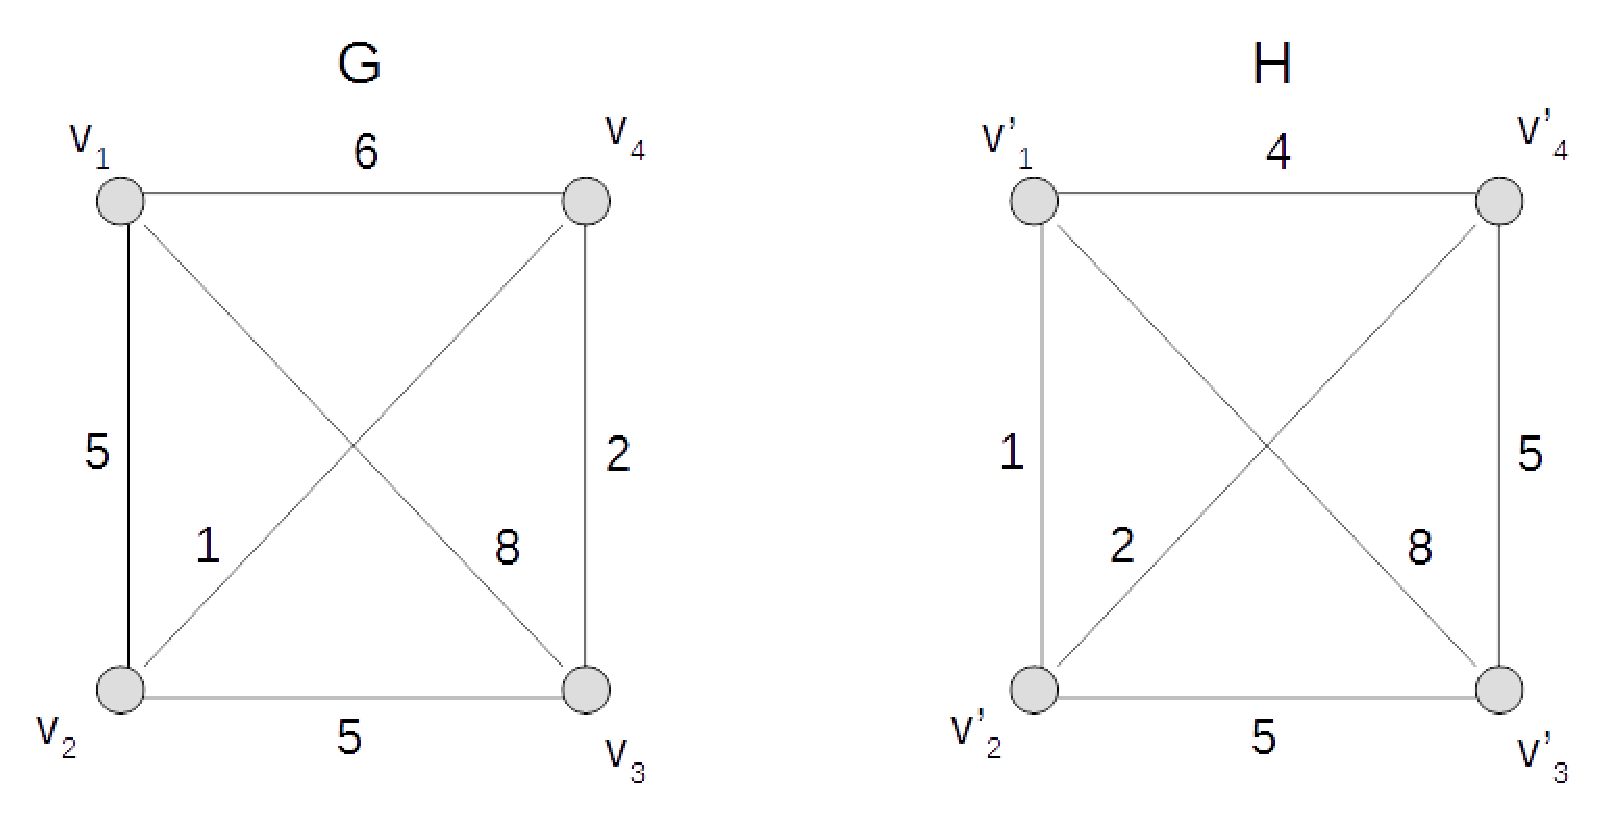
\includegraphics[width=12.5cm]{../images/gh.eps}
  \caption{グラフG、グラフH}
\end{figure}

図のグラフから隣接行列$A_G$、$A_H$は以下のようになる。
\begin{eqnarray}
  A_G=\begin{pmatrix}
    0.0 & 5.0 & 8.0 & 6.0 \\
    5.0 & 0.0 & 5.0 & 1.0 \\
    8.0 & 5.0 & 0.0 & 2.0 \\
    6.0 & 1.0 & 2.0 & 0.0
  \end{pmatrix} \notag \\
  A_H=\begin{pmatrix}
    0.0 & 1.0 & 8.0 & 4.0 \\
    1.0 & 0.0 & 5.0 & 2.0 \\
    8.0 & 5.0 & 0.0 & 5.0 \\
    4.0 & 2.0 & 5.0 & 0.0
  \end{pmatrix} \notag
\end{eqnarray}

得られた行列$A_G$、$A_H$をそれぞれ固有値分解する。この時、固有ベクトルを、対応する固有値の大きさ順に並べたモード行列を$U_G$、$U_H$とし、固有値を大きい順に対角上に並べた対角行列を$\Lambda_G$、$\Lambda_H$とすると以下の式のように表せる。
\begin{gather}
  \label{gaul}
  A_G=U_G\Lambda_GU_G^T \\
  \Lambda_G=diag(14.25,-0.28,-4.83,-9.14) \notag \\
  U_G=\begin{pmatrix}
    0.614 & 0.141 & -0.182 & -0.755 \\
    0.434 & -0.528 & 0.726 & 0.079 \\
    0.548 & -0.270 & -0.582 & 0.536 \\
    0.366 & 0.793 & 0.371 & 0.369
  \end{pmatrix} \notag \\
    \label{haul}
    A_H=U_H\Lambda_HU_H^T \\
    \Lambda_H=diag(13.26,-0.77,-3.43,-9.05) \notag \\
    U_H=\begin{pmatrix}
      0.538 & -0.436 & -0.425 & -0.583 \\
      0.344 & 0.880 & -0.018 & -0.327 \\
      0.624 & 0.026 & -0.250 & 0.740 \\
      0.450 & 0.187 & 0.870 & 0.079
    \end{pmatrix} \notag
\end{gather}
$U_G$、$U_H$のすべての要素の絶対値を取ると、行に各ノード、列に各固有値ベクトルが対応させることができる。
\begin{gather}
  \overline{U}_G=\begin{pmatrix}
    0.614 & 0.141 & 0.182 & 0.755 \\
    0.434 & 0.528 & 0.726 & 0.079 \\
    0.548 & 0.270 & 0.582 & 0.536 \\
    0.366 & 0.793 & 0.371 & 0.369
  \end{pmatrix} \notag \\
  \overline{U}_H=\begin{pmatrix}
    0.538 & 0.436 & 0.425 & 0.583 \\
    0.344 & 0.880 & 0.018 & 0.327 \\
    0.624 & 0.026 & 0.250 & 0.740 \\
    0.450 & 0.187 & 0.870 & 0.079
  \end{pmatrix} \notag
\end{gather}
行に各ノードというのはつまり、ノード数4の重み付き無向グラフを、隣接行列の固有値分解により4次元空間上で重みを距離に反映した四つの頂点に変換したことになる。

$A_G$と$A_H$が同型であると仮定すると、式(\ref{jp_p2})の左辺が0になる。よって、
\begin{equation}
  \label{pageah}
  PA_GP^T=A_H
\end{equation}
を満たす$P$が存在する。式(\ref{pageah})、(\ref{gaul})、(\ref{haul})より、
\begin{equation}
  PU_G\Lambda_GU_G^TP^T=U_H\Lambda_hU_H^T \notag
\end{equation}
再度、$A_G$、$A_H$が同型であるという仮定から
\begin{equation}
  PU_G=U_HS \notag
\end{equation}
を満たす行列$S$が存在し、
\begin{equation}
  P=U_HSU_G^T \notag
\end{equation}
と表せる。

求めたい$P$は順列行列であるから、$\hat{P}$を導入し、
\begin{eqnarray}
  \hat{P}=\bordermatrix{  & & \pi(i) \cr
                    & & \vdots \cr
                  i & \cdots & 1 \cr
                  } \notag
\end{eqnarray}
対角行列を$\hat{S}$とし、$U_H=[h_{ij}]$、$U_G=[g_{ij}]$、$\hat{S}=diag(s_i)$であることを用いて
\begin{equation}
  tr(\hat{P}^TU_H\hat{S}U_G^T)=\textstyle\sum\limits_{i=1}^{n}\textstyle\sum\limits_{j=1}^{n}s_jh_{ij}g_{\pi(i)j} \notag
\end{equation}
ここで、
\begin{equation}
  \begin{split}
  \sum_{j=1}^{n}s_jh_{ij}g_{\pi(i)j}&\le|\textstyle\sum\limits_{j=1}^{n}s_jh_{ij}g_{\pi(i)j} \notag \\
                                    &\le\textstyle\sum\limits_{j=1}^{n}|s_jh_{ij}g_{\pi(i)j} \notag \\
                                    &=\textstyle\sum\limits_{j=1}^{n}|h_{ij}||g_{\pi(i)j} \notag
  \end{split}
\end{equation}
よって、
\begin{equation}
  \begin{split}
    tr(\hat{P}^TU_H\hat{s}U_G^T)&\le\textstyle\sum\limits_{i=1}^{n}\textstyle\sum\limits_{j=1}^{n}|h_{ij}||g_{\pi(i)j}| \notag \\
          &=tr(\hat{P}\overline{U}_H\overline{U}_G^T) \notag
  \end{split}
\end{equation}

モード行列$U_G$、$U_H$は長さ1の固有ベクトルでできた行列であり、各要素の絶対値を取った$\overline{U}_G$、$\overline{U}_H$の行ベクトルも長さは1であるから、$\overline{U}_G\overline{U}_H=[x_{ij}]$とした時、$0\le x_{ij}\le1$を満たす。

以上より、任意の順列行列$P$は、
\begin{equation}
  tr(P^T\overline{U}_H\overline{U}_G^T)\le n \notag
\end{equation}
を満たし、$P$が最適マッチングを導く時、$n$が最大値となるので、$\overline{U}_H\overline{U}_G^T$に、ハンガリアン法を用いることで、最適な割り当てを求めている。

参考までに、ハンガリアン法を用いて求められた$P$は、
\begin{equation}
  P=\begin{pmatrix}
    0 & 0 & 1 & 0 \\
    0 & 0 & 0 & 1 \\
    1 & 0 & 0 & 0 \\
    0 & 1 & 0 & 0
  \end{pmatrix} \notag
\end{equation}

\subsection{ハンガリアン法}
\textbf{ハンガリアン法}(Hungarian method)とは、割当問題の解法として頻繁に用いられるものの一つであり、n次の正方行列が与えられた時、それぞれの行、列に重複が無いように値を選び出し、最小となる組合せを見つけるといった問題を解くことができる。たとえば、「n個の仕事をn人の作業員にやらせる時のコストを考える。同じ仕事を複数人の作業員でこなすことは無く、また、同じ作業員が複数の仕事をこなすこともないことを条件とし、仕事jを作業員iがやる時のコストを$c_{ij}$としたコスト行列Cを入力として、コストが最小になる割り当てを見つける」

グラフのノードマッチングを解く際は、最大となる組合せを見つけることになるが、予め行列の全要素を-1倍してから最小となる組合せを見つけることにし、最大化問題を最小化問題に置き換えている。

ハンガリアン法は、以下の6ステップにより構成される。
\begin{enumerate}
  \item 各行の最小値を、その行の全要素から引く。
  \item 各列の最小値を、その列の全要素から引く。
  \item 行列内のすべての0を通るように必要最小限数の直線を引き、直線状の要素に印をつける。
  \item $直線の本数=n$であれば、値が0の要素が最適マッチングの位置であり、終了。
  \item $直線の本数<n$であれば、印のないすべての要素の最小値を、印がないすべての要素から引き、印が二つついている要素には同じ値を加算する。
  \item 4に戻る。
\end{enumerate}
作業員に割り当てる際、作業員毎のコストの差が重要であり、差が同じであれば最適な割当ては変わらない点に注目している。

\subsection{まとめ}
梅山氏の提案手法で想定されている入力は、ノード数が一致しており、構造がほぼ同型なグラフであり、それ以外の、ノード数が一致しなかったり、グラフの構造が大きく異なっているもの同士のノードマッチングの精度は保証されないことに注意する必要がある。
